\documentclass[12pt,a4paper]{article}
\usepackage{here}
\usepackage{amsmath,amscd,amsbsy,amssymb,latexsym,url,bm,amsthm}
\usepackage{epsfig,graphicx,subfigure}
\usepackage{enumitem,balance}
\usepackage{wrapfig}
\usepackage{mathrsfs,euscript}
\usepackage[usenames]{xcolor}
\usepackage{hyperref}
\usepackage[vlined,ruled,linesnumbered]{algorithm2e}
\usepackage{array}
\hypersetup{colorlinks=true,linkcolor=black}

\newtheorem{theorem}{Theorem}
\newtheorem{lemma}[theorem]{Lemma}
\newtheorem{proposition}[theorem]{Proposition}
\newtheorem{corollary}[theorem]{Corollary}
\newtheorem{exercise}{Exercise}
\newtheorem*{solution}{Solution}
\newtheorem{definition}{Definition}
\theoremstyle{definition}

\renewcommand{\thefootnote}{\fnsymbol{footnote}}

\newcommand{\postscript}[2]
 {\setlength{\epsfxsize}{#2\hsize}
  \centerline{\epsfbox{#1}}}

\renewcommand{\baselinestretch}{1.0}

\setlength{\oddsidemargin}{-0.365in}
\setlength{\evensidemargin}{-0.365in}
\setlength{\topmargin}{-0.3in}
\setlength{\headheight}{0in}
\setlength{\headsep}{0in}
\setlength{\textheight}{10.1in}
\setlength{\textwidth}{7in}
\makeatletter \renewenvironment{proof}[1][Proof] {\par\pushQED{\qed}\normalfont\topsep6\p@\@plus6\p@\relax\trivlist\item[\hskip\labelsep\bfseries#1\@addpunct{.}]\ignorespaces}{\popQED\endtrivlist\@endpefalse} \makeatother
\makeatletter
\renewenvironment{solution}[1][Solution] {\par\pushQED{\qed}\normalfont\topsep6\p@\@plus6\p@\relax\trivlist\item[\hskip\labelsep\bfseries#1\@addpunct{.}]\ignorespaces}{\popQED\endtrivlist\@endpefalse} \makeatother

\begin{document}
\noindent

%========================================================================
\noindent\framebox[\linewidth]{\shortstack[c]{
\Large{\textbf{Lab10-Turing Machine}}\vspace{1mm}\\
CS214-Algorithm and Complexity, Xiaofeng Gao \& Lei Wang, Spring 2021.}}
\begin{center}
\footnotesize{\color{red}$*$ If there is any problem, please contact TA Yihao Xie. }

\footnotesize{\color{blue}$*$ Name:Beichen Yu \quad Student ID:519030910245 \quad Email: polarisybc@sjtu.edu.cn}
\end{center}

\begin{enumerate}
    \item Design a one-tape TM $M$ that computes the function $f(x, y) = \lfloor x/y \rfloor$, where $x$ and $y$ are positive integers $(x > y)$. The alphabet is $\{1, 0, \Box, \triangleright, \triangleleft\}$, and the inputs are $x$ "1"s, $\Box$ and $y$ "1"s. Below is the initial configuration for input $x=7$ and $y=3$. The result $z=f(x,y)$ should also be represented in the form of $z$ "1"s on the tape with pattern of $\rhd 111\cdots 111\lhd$, which is $\rhd 11\lhd$ for the example.
    
	\begin{center}
		\begin{tabular}{ll|c|c|c|c|c|c|c|c|c|c|c|c|c|c}
			& \multicolumn{14}{c}{Initial Configuration}\\[5pt]
			\cline{2-16}
			& & $\triangleright$ &  1  & 1 & 1 & 1 & 1 & 1 & 1 & $\Box$ & 1 & 1 & 1 & $ \triangleleft$ & \\
			\cline{2-16}
			\multicolumn{2}{c}{} & \multicolumn{1}{c}{$\uparrow$} & \multicolumn{11}{c}{}\\[-4px]
			\multicolumn{2}{c}{} & \multicolumn{1}{c}{$q_S$} & \multicolumn{11}{c}{}	
		\end{tabular}
	\end{center}

    \begin{enumerate}
	\item
	Please describe your design and then write the specifications of $M$ in the form like $\langle q_S, \triangleright \rangle \rightarrow \langle q_1, \triangleright,  R\rangle$. Explain the transition functions in detail.
	
	\item
	Please draw the state transition diagram.
	
	\item
	Show briefly and clearly the whole process from initial to final configurations for input $x = 7$ and $y = 3$. You may start like this:
	$$(q_s,\underline{\triangleright}  1  1  1  1  1  1  1  \Box 1  1  1   \triangleleft)
	\vdash (q_1,\triangleright  \underline{1}  1  1  1  1  1  1  \Box 1  1  1   \triangleleft)
	\vdash^* (q_1,\triangleright  1  1  1  1  1  1  1  \underline{\Box} 1  1  1   \triangleleft)
	\vdash (q_2,\triangleright  1  1  1  1  1  1  1  \Box \underline{1}  1  1   \triangleleft)$$
	
	\par{\color{blue}(Note that for simplicity, we write $(q_1,\triangleright  \underline{1}  1  1  1  1  1  1  \Box 1  1  1   \triangleleft)\vdash^* (q_1,\triangleright  1  1  1  1  1  1  1  \underline{\Box} 1  1  1   \triangleleft)$ if the corresponding transaction repeats on multiple inputs with the same state.)}
\end{enumerate}
	\begin{solution}
		\begin{enumerate}
			\item 
			Start state:
			\begin{align*}
			\langle q_S, \triangleright \rangle \rightarrow \langle q_1, \triangleright,  R\rangle
			\end{align*}
			Go to the first ``1'' of $ y $:	
			\begin{align*}
				\langle q_1, 1 \rangle &\rightarrow \langle q_1, 1,  R\rangle \\
				\langle q_1, \Box \rangle &\rightarrow \langle q_2, \Box,  R\rangle
			\end{align*}
			Change all ``1'' of $ y $ into 0, while delete the same number of ``1'' in $ x $:
			\begin{align*}
				\langle q_2, 1 \rangle &\rightarrow \langle q_3, 0,  L\rangle \\
				\langle q_3, 0 \rangle &\rightarrow \langle q_3, 0,  L\rangle \\
				\langle q_3,\Box \rangle &\rightarrow \langle q_3, \Box ,  L\rangle \\
				\langle q_3,1 \rangle &\rightarrow \langle q_2, \Box ,  R\rangle \\
				\langle q_2,\Box \rangle &\rightarrow \langle q_2, \Box ,  R\rangle \\
				\langle q_2,0 \rangle &\rightarrow \langle q_2, 0 ,  R\rangle 
			\end{align*}
			Write a ``1'' in the right side of $ \triangleleft $, and turn all ``0'' back to ``1'':
			\begin{align*}
				\langle q_2, \triangleleft \rangle &\rightarrow \langle q_4, \triangleleft,  R\rangle \\
				\langle q_4, 1 \rangle &\rightarrow \langle q_4, 1,  R\rangle\\
				\langle q_4, \Box \rangle &\rightarrow \langle q_5, 1,  L\rangle\\
				\langle q_5, 1 \rangle &\rightarrow \langle q_5, 1,  L\rangle\\
				\langle q_5, \triangleleft \rangle &\rightarrow \langle q_5, \triangleleft,  L\rangle\\
				\langle q_5, 0 \rangle &\rightarrow \langle q_5, 1,  L\rangle\\
				\langle q_5, \Box \rangle &\rightarrow \langle q_2, \Box,  R\rangle
			\end{align*}
			If the remain ``1'' in $ x $ is less than the number of ``1'' in $ y $, end the loop and get the answer:
			\begin{align*}
				\langle q_3, \triangleright  \rangle &\rightarrow \langle q_6, \Box,  R\rangle \\
				\langle q_6, 1  \rangle &\rightarrow \langle q_6, \Box,  R\rangle \\
				\langle q_6, \Box \rangle &\rightarrow \langle q_6, \Box,  R\rangle \\
				\langle q_6, 0  \rangle &\rightarrow \langle q_6, \Box,  R\rangle \\
				\langle q_6, \triangleleft  \rangle &\rightarrow \langle q_7, \triangleright,  R\rangle \\
				\langle q_7, 1  \rangle &\rightarrow \langle q_7, 1,  R\rangle \\
				\langle q_7, \Box \rangle &\rightarrow \langle q_H, \triangleleft,  R\rangle 
			\end{align*}

			\item Below is the state transition diagram.
			\begin{figure}[H]
				\centering
				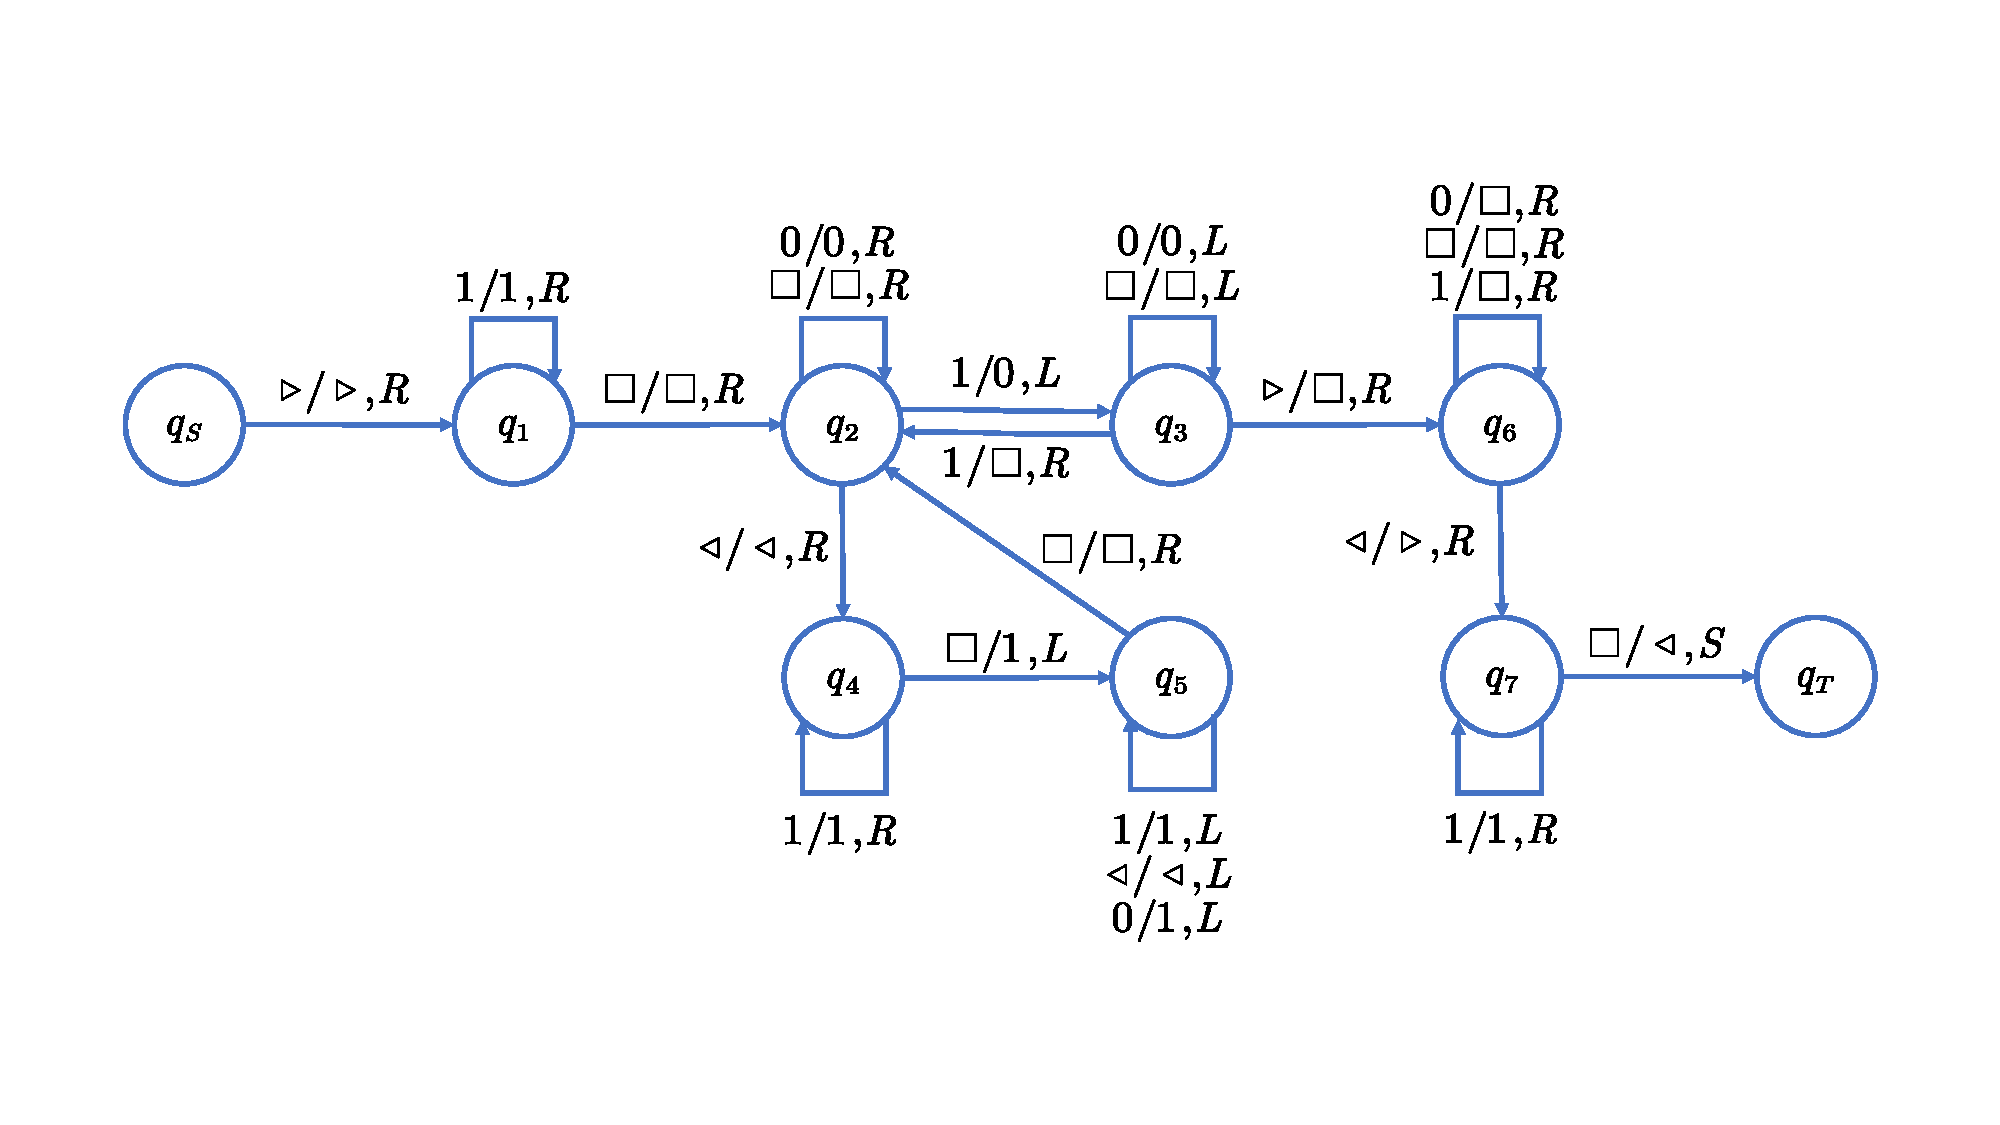
\includegraphics[width=\textwidth]{std.pdf}
				\caption{The state transition diagram}
				\end{figure}

			\item 
			\begin{align*}
				&(q_s,\underline{\triangleright}  1  1  1  1  1  1  1  \Box 1  1  1   \triangleleft)\\
				\vdash &(q_1,\triangleright  \underline{1}  1  1  1  1  1  1  \Box 1  1  1   \triangleleft)\\
				\vdash^* &(q_1,\triangleright  1  1  1  1  1  1  1  \underline{\Box} 1  1  1   \triangleleft)\\		
				\vdash &(q_2,\triangleright  1  1  1  1  1  1  1  \Box \underline{1}  1  1   \triangleleft)\\
				\vdash &(q_3,\triangleright  1  1  1  1  1  1  1  \underline{\Box} 0  1  1   \triangleleft)	\\
				\vdash &(q_3,\triangleright  1  1  1  1  1  1  \underline{1} \Box 0  1  1   \triangleleft)\\
				\vdash &(q_2,\triangleright  1  1  1  1  1  1  \Box \underline{\Box}  0  1  1   \triangleleft)\\	
				\vdash &(q_2,\triangleright  1  1  1  1  1  1  \Box \Box \underline{0}  1  1   \triangleleft)\\		
				\vdash &(q_2,\triangleright  1  1  1  1  1  1  \Box \Box  0 \underline{1}  1   \triangleleft)\\
				\vdash^* &(q_2,\triangleright  1  1  1  1   \Box \Box  \Box \Box  0  0  \underline{0}   \triangleleft)\\
			\end{align*}
			\begin{align*}
				\vdash  &(q_2,\triangleright  1  1  1  1   \Box \Box  \Box \Box  0  0  0  \underline{\triangleleft})\\
				\vdash  &(q_4,\triangleright  1  1  1  1   \Box \Box  \Box \Box  0  0  0 \triangleleft \underline{\Box})\\
				\vdash  &(q_5,\triangleright  1  1  1  1   \Box \Box  \Box \Box  0  0  0  \underline{\triangleleft} 1)\\
				\vdash  &(q_5,\triangleright  1  1  1  1   \Box \Box  \Box \Box  0  0  \underline{0}  \triangleleft 1)\\
				\vdash  &(q_5,\triangleright  1  1  1  1   \Box \Box  \Box \Box  0  \underline{0} 1 \triangleleft 1)\\
				\vdash^*  &(q_5,\triangleright  1  1  1  1   \Box \Box  \Box \underline{\Box}  1  1  1  \triangleleft 1)\\
				\vdash  &(q_2,\triangleright  1  1  1  1   \Box \Box  \Box \Box   \underline{1} 1 1 \triangleleft 1)\\
				\vdash^* &(q_2,\triangleright  1  \Box \Box  \Box \Box \Box  \Box \Box   \underline{1} 1 1 \triangleleft 1 1)\\
				\vdash^* &(q_3,\underline{\triangleright}  \Box \Box \Box  \Box \Box \Box  \Box \Box 1 1 1 \triangleleft 1 1)\\
				\vdash &(q_6, \Box \underline{\Box} \Box \Box  \Box \Box \Box  \Box \Box 1 1 1 \triangleleft 1 1)\\
				\vdash^* &(q_6, \underline{1} 1 1 \triangleleft 1 1)\\
				\vdash &(q_6, \Box \underline{1} 1 \triangleleft 1 1)\\
				\vdash^* &(q_6, \underline{\triangleleft} 1 1)\\
				\vdash &(q_7, \triangleright \underline{1} 1)\\
				\vdash &(q_7, \triangleright 1 \underline{1})\\
				\vdash &(q_7, \triangleright 1 1 \underline{\Box})\\
				\vdash &(q_T, \triangleright 1 1 \underline{\triangleleft})
			\end{align*}

			
		\end{enumerate}
	\end{solution}


    \item 
    Given the alphabet $\{1, 0, \Box, \triangleright, \triangleleft\}$, design a time efficient 3-tape TM $M$ to compute $f:\{0,1\}^*\rightarrow\{0,1\}$ which verifies whether the number of 0 and the number of 1 are the same in an input consisting of only 0's and 1's. $M$ should output 1 if the numbers are the same, and 0 otherwise. For eample, for the input tape $\triangleright 001101\triangleleft$, $M$ should output 1
    
    \begin{enumerate}
	    \item
	    Please describe your design and then write the specifications of $M$ in the form like $\langle q_S, \triangleright, \triangleright, \triangleright \rangle \rightarrow \langle q_1, \triangleright,\triangleright,  R, R, S \rangle$. Explain the transition functions in detail.
	    
	    \item 
	    Show the time complexity for one-tape TM $M'$ to compute the same function $f$ with $n$ symbols in the input and give a brief description of such $M'$ .
	
	\end{enumerate}
	
	\begin{solution}
		\begin{enumerate}
			\item Start state:
			\begin{align*}
				\langle q_S, \triangleright, \triangleright, \triangleright \rangle \rightarrow \langle q_1, \triangleright,\triangleright,  R, R, S \rangle
			\end{align*}
			Go right, write a ``1'' in the second tape if it reads a ``1'' in the first tape, and do nothing if reads ``0'' in the first tape:
			\begin{align*}
				\langle q_1, 0, \Box, \triangleright \rangle &\rightarrow \langle q_1, \Box,\triangleright,  R, S, S \rangle\\
				\langle q_1, 1, \Box, \triangleright \rangle &\rightarrow \langle q_1, 1,\triangleright,  R, R, S \rangle\\
				\langle q_1, \triangleleft, \Box, \triangleright \rangle &\rightarrow \langle q_2, \Box, \triangleright,  L, L, S \rangle\\
			\end{align*}
			Go left, move to left in the second tape if it reads a ``0'' in the first tape, and do nothing if reads ``1'' in the first tape:
			\begin{align*}
				\langle q_2, 1, 1, \triangleright \rangle &\rightarrow \langle q_2, 1,\triangleright,  L, S, S \rangle\\
				\langle q_2, 0, 1, \triangleright \rangle &\rightarrow \langle q_2, 1,\triangleright,  L, L, S \rangle\\
			\end{align*}
			If the first tape and the second tape meet $ \triangleright $ together, then the number of 0 and the number of 1 are the same:
			\begin{align*}
				\langle q_2, \triangleright, \triangleright, \triangleright \rangle &\rightarrow \langle q_4, \triangleright,\triangleright,  S, S, R \rangle\\
				\langle q_4, \triangleright, \triangleright, \Box \rangle &\rightarrow \langle q_5, \triangleright,1,  S, S, R \rangle\\
				\langle q_5, \triangleright, \triangleright, \Box \rangle &\rightarrow \langle q_H, \triangleright,\triangleleft,  S, S, S \rangle\\
			\end{align*}
			Otherwise, then the number of 0 and the number of 1 are not the same:
			\begin{align*}
				\langle q_2, 0, \triangleright, \triangleright \rangle &\rightarrow \langle q_6, \triangleright,\triangleright,  S, S, R \rangle\\
				\langle q_2, 1, \triangleright, \triangleright \rangle &\rightarrow \langle q_6, \triangleright,\triangleright,  S, S, R \rangle\\
				\langle q_2,  \triangleright, 1,\triangleright \rangle &\rightarrow \langle q_6, 1,\triangleright,  S, S, R \rangle\\
				\langle q_6, 0, \triangleright, \Box \rangle &\rightarrow \langle q_7, \triangleright,0,  S, S, R \rangle\\
				\langle q_6, 1, \triangleright, \Box \rangle &\rightarrow \langle q_7, \triangleright,0,  S, S, R \rangle\\
				\langle q_6,  \triangleright,1, \Box \rangle &\rightarrow \langle q_7, 1,0,  S, S, R \rangle\\
				\langle q_7, 0, \triangleright, \Box \rangle &\rightarrow \langle q_H, \triangleright,\triangleleft,  S, S, S \rangle\\
				\langle q_7, 1, \triangleright, \Box \rangle &\rightarrow \langle q_H, \triangleright,\triangleleft,  S, S, S \rangle\\
				\langle q_7, \triangleright, 1, \Box \rangle &\rightarrow \langle q_H, 1,\triangleleft,  S, S, S \rangle\\
			\end{align*}
			\item The $ M' $ can use the similar algorithm with the $ M $. Each time the reading head reads a ``1'', it moves to the right side and write a flag; after it goes to the rightest side, then turn left. In this turn, each time the reading head reads a ``0'', it moves to the right side and delete a flag. Then it can make a compare according to the number of flags. 
			
			Because the time complexity of moving right is $ O(n) $ and there are $ n $ symbols in the input, the final time complexity is $ O(n^2) $.
		\end{enumerate}
	\end{solution}
	\item Define the corresponding decision or search problem of the following problems and give the "certificate" and "certifier" for each decision problem provided in the subquestions or defined by yourself.
	
	\begin{enumerate}
	    \item
	    \textit{3-Dimensional Matching.}  Given disjoint sets $X,Y,Z$ all with the size of $n$, and a set $M \subseteq X\times Y\times Z$.  Is there a subset $M'$ of $M$ of size $n$ where no two elements of $M'$ agree in any coordinate?
	    
	    \item 
	    \textit{Travelling Salesman Problem.} Given a list of cities and the distances between each pair of cities, find the shortest possible route that visits each city exactly once and returns to the origin city.
	    
	    \item
	    \textit{Job Sequencing.} Given a set of unit-time jobs, each of which has an integer deadline and a nonnegative penalty for missing the deadline. Does there exist a job sequence that has a total penalty $w\leqslant k$?
	    
	\end{enumerate}

	\begin{solution}
		\begin{enumerate}
			\item This is a decision problem.
			
			The search problem is: Find a subset $M'$ of $M$ of size $n$ where no two elements of $M'$ agree in any coordinate.

			\textit{Certificate:} A subset $M'$ of $M$ of size $n$.
			
			\textit{Certifier:} Check that in any coordinate there are no two elements of $M'$ agree.

			\item This is a search problem.
			
			The decision problem is: Is there a route that visits each city exactly once and returns to the origin city and its length $ l \leqslant k $.
			
			\textit{Certificate:} A route $ r_0 $ that visits each city exactly once and returns to the origin city.
			
			\textit{Certifier:} Assume that the length of $ r_0 $ is $ l_0 $. Check that $ l_0 \leqslant  k$. 

			\item This is a decision problem.
			
			The search problem is: Find a job sequence with a smallest total penalty.
			
			
			\textit{Certificate:} A job sequence $ s $.
			
			\textit{Certifier:} Check that the total penalty $w$ of $ s $ is less or equal to $ k $.

		\end{enumerate}
	\end{solution}

\end{enumerate}

\textbf{Remark:} Please include your .pdf, .tex files for uploading with standard file names.
\newpage


%========================================================================
\end{document}